\section{ARM64 Architecture}

ARM64 (AArch64) is a 64-bit architecture developed by ARM Holdings, widely used in modern mobile devices and servers.\par
ARM64 offers a significant register file structure, with 31 general-purpose registers and special-purpose registers such as the Program Counter (PC) and Stack Pointer (SP). These registers provide flexibility for performing low-level operations efficiently.

\paragraph{Key Features}
\begin{itemize}
	\item 64-bit general-purpose registers (X0-X30).
	\item Special-purpose registers for the stack, program control, and more.
	\item Optimized function calling convention.
\end{itemize}
\subsection{Memory Layout in Computer Systems}

In modern computer systems, memory is divided into several distinct segments that each serve a different purpose in the execution of a program. These segments include the stack, heap, and various regions that hold code and data. This section provides a mathematical description of the layout of memory in a typical system and explains the role of each memory segment.

\subsubsection{Memory Segments}

A typical program is divided into the following memory segments:

\begin{table}[h]
	\centering
	\begin{tabular}{|c|l|}
		\hline
		\multirow{2}{*}{\textbf{Stack}} & Used for local variables, function call management, and control flow. \\
		& It grows downward in memory. \\ \hline
		\multirow{2}{*}{\textbf{Heap}} & Used for dynamic memory allocation (e.g., via \texttt{malloc}). \\ & It grows upward in memory. \\ \hline
		\textbf{.text} & Stores the program's executable instructions (machine code). \\ \hline
		\textbf{.data} & Stores initialized global and static variables. \\ \hline
		\multirow{2}{*}{\textbf{.bss}} & Stores uninitialized global and static variables. \\
		& This segment is initialized to zero at runtime. \\ \hline
		\textbf{.rodata} & Stores read-only data, such as string literals or constant variables. \\ \hline
	\end{tabular}
	%	\caption{Summary of memory segments in a typical program.}
\end{table}
\begin{itemize}
	\item \textbf{Stack:} Used for local variables, function call management, and control flow. It grows downward in memory.
	\item \textbf{Heap:} Used for dynamic memory allocation (e.g., via \texttt{malloc}). It grows upward in memory.
	\item \textbf{.text:} Stores the program's executable instructions (machine code).
	\item \textbf{.data:} Stores initialized global and static variables.
	\item \textbf{.bss:} Stores uninitialized global and static variables. This segment is initialized to zero at runtime.
	\item \textbf{.rodata:} Stores read-only data, such as string literals or constant variables.
\end{itemize}

\noindent The memory layout in a typical process can be visualized as:

\begin{center}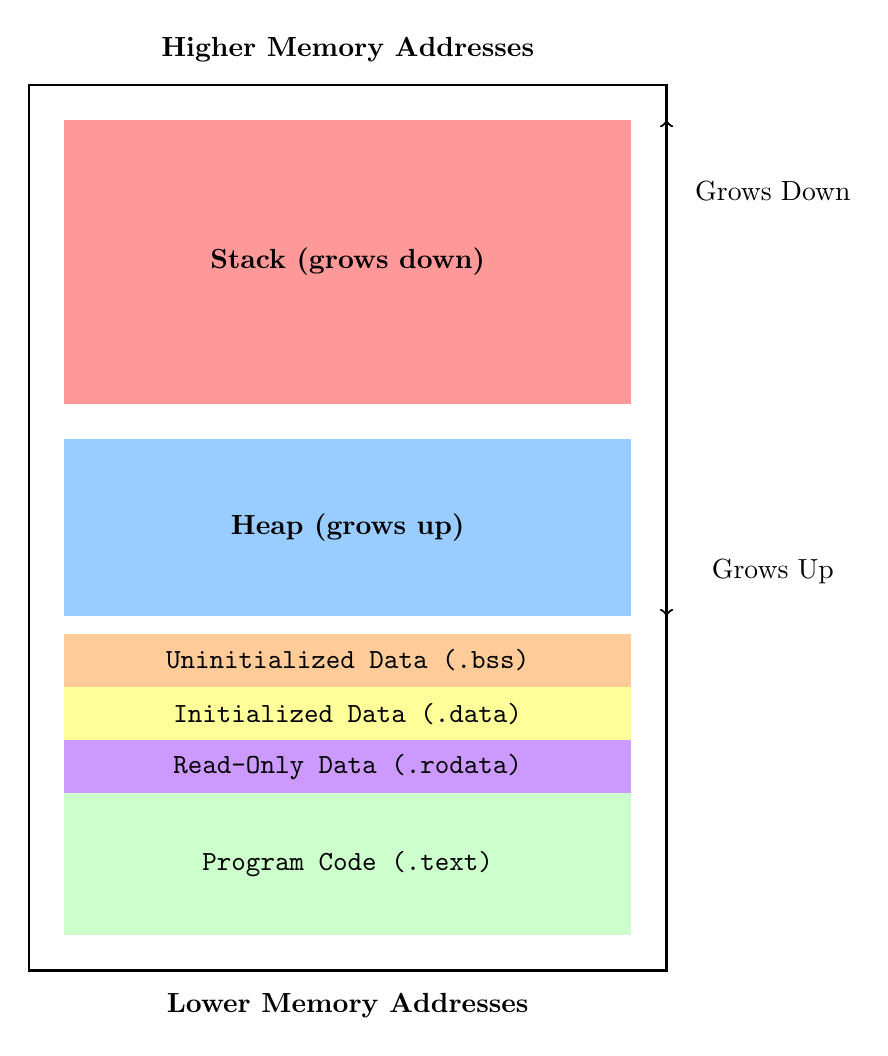
\begin{tikzpicture}[scale=.9]
		% Define colors for segments
		\definecolor{stackcolor}{RGB}{255, 153, 153}
		\definecolor{heapcolor}{RGB}{153, 204, 255}
		\definecolor{textcolor}{RGB}{204, 255, 204}
		\definecolor{datacolor}{RGB}{255, 255, 153}
		\definecolor{bsscolor}{RGB}{255, 204, 153}
		\definecolor{rodatacolor}{RGB}{204, 153, 255}
		
		% Base address
		\node at (0,10.5) {\textbf{Higher Memory Addresses}};
		\node at (0,-3.0) {\textbf{Lower Memory Addresses}};
		
		% Expanded width for rectangles (from -4 to 4)
		% Stack
		\fill[stackcolor] (-4, 5.5) rectangle (4, 9.5);
		\node at (0,7.5) {\textbf{Stack (grows down)}};
		
		% Heap
		\fill[heapcolor] (-4, 2.5) rectangle (4, 5);
		\node at (0,3.75) {\textbf{Heap (grows up)}};
		
		% BSS
		\fill[bsscolor] (-4, 1.5) rectangle (4, 2.25);
		\node at (0,1.875) {\texttt{Uninitialized Data (.bss) }};
		
		% Data
		\fill[datacolor] (-4, 0.75) rectangle (4, 1.5);
		\node at (0,1.125) {\texttt{Initialized Data (.data)}};
		
		% ROData
		\fill[rodatacolor] (-4, 0) rectangle (4, 0.75);
		\node at (0,0.375) {\texttt{Read-Only Data (.rodata)}};
		
		% Text
		\fill[textcolor] (-4, -2) rectangle (4, 0);
		\node at (0,-1) {\texttt{Program Code (.text)}};
		
		% Annotations and arrows
		\draw[thick,->] (4.5,7.5) -- (4.5,9.5);
		\node at (6,8.5) {Grows Down};
		
		\draw[thick,->] (4.5,3.75) -- (4.5,2.5);
		\node at (6,3.125) {Grows Up};
		
		% Memory boundary lines (Expand to match rectangle width)
		\draw[thick] (-4.5, -2.5) rectangle (4.5, 10);
\end{tikzpicture}\end{center}
\newpage
\subsection{Performance Metrics and Benchmarks}
A computer user focuses on minimizing \textbf{response time} (or \textbf{execution time}), while a warehouse-scale operator aims to maximize \textbf{throughput}, the total work completed in a given period.\sidenote{John L. Hennessy and David A. Patterson,
	\textit{Computer Architecture: A Quantitative Approach},
	5th ed., Morgan Kaufmann, 2011.}

We want to relate the performance of two different computers, say, $X$ and $Y$. For the phase \begin{center}
``$X$ is faster than $Y$'',
\end{center} we can define it in terms of execution times: let
\begin{itemize}
	\item \( T_X \) denote the execution time of computer \( X \),
	\item \( T_Y \) denote the execution time of computer \( Y \).
\end{itemize} If \( X \) is faster than \( Y \), then:
\[
T_X < T_Y
\]
This inequality means that the time required for \( X \) to complete the task is less than the time required for \( Y \).

In particular, ``$X$ is $n$ times faster than $Y$''\sidenote{
The computer $X$ is 1.5 times faster than $Y$ means that \[
1.5=\frac{\text{Execution Time}_Y}{\text{Execution Time}_X}.
\] If $\text{Execution Time}_X=10$s and $\text{Execution Time}_Y=15$s, TFAE:
\begin{itemize}
	\item $X$ is 1.5 times faster than $Y$
	\item $Y$ is about 0.76 times slower than $X$.
\end{itemize}
} means that \[
\frac{\text{Execution Time}_Y}{\text{Execution Time}_X}=n.
\] Since execution time is the reciprocal of performance, the following relationship holds:
\[
n = \frac{\text{Execution Time}_Y}{\text{Execution Time}_X} =\frac{\displaystyle 1/\text{Performance}_Y}{\displaystyle 1/\text{Performance}_X}= \frac{\text{Performance}_X}{\text{Performance}_Y}.
\]
where: \begin{itemize}
	\item \( n > 1 \): Computer \( X \) is \( n \) times faster than \( Y \).
	\item \( n < 1 \): Computer \( X \) is \( 1/n\) times slower than \( Y\). In other words, computer $Y$ is $1/n$ times faster than computer $X$.
\end{itemize} 

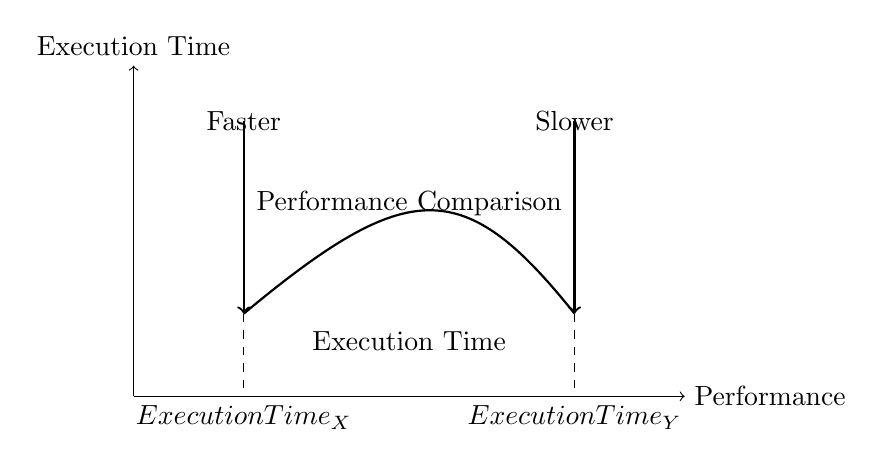
\begin{tikzpicture}[scale=0.7]
	\draw[->] (0,0) -- (10,0) node[right] {Performance};
	\draw[->] (0,0) -- (0,6) node[above] {Execution Time};
	
	\node[align=center] at (2,5) {Faster};
	\node[align=center] at (8,5) {Slower};
	
	\draw[thick, ->] (2,5) -- (2,1.5);
	\draw[thick, ->] (8,5) -- (8,1.5);
	
	% Dotted line for Execution Time X
	\draw[dashed] (2,1.5) -- (2,0) node[below] {$\text{Execution Time}_X$};
	\draw[dashed] (8,1.5) -- (8,0) node[below] {$\text{Execution Time}_Y$};
	
	% Execution Time labels
	\node[align=center] at (5,1) {Execution Time};
	
	% Performance Curve
	\draw[thick] (2,1.5) .. controls (5,4) and (6,4) .. (8,1.5);
	
	% Performance Label
	\node[align=center] at (5,3.5) {Performance Comparison};
\end{tikzpicture}
\newpage
\subsubsection{Quantifying Performance}

Understanding performance is crucial in evaluating computer systems. We use metrics such as \textbf{response time} (or \textit{execution time}) and \textbf{throughput} to measure the efficiency of a system. The relationship between performance and execution time is inversely proportional:
\[
\text{Performance} = \frac{1}{\text{Execution Time}}
\]

This relationship allows us to compare two systems, X and Y:
\[
\text{n} = \frac{\text{Performance}_X}{\text{Performance}_Y} = \frac{\text{Execution Time}_Y}{\text{Execution Time}_X}
\]

\subsubsection{Illustrating Performance Comparison}

The following diagram represents the comparison between two systems, X and Y, in terms of their execution time and throughput:

\begin{center}
	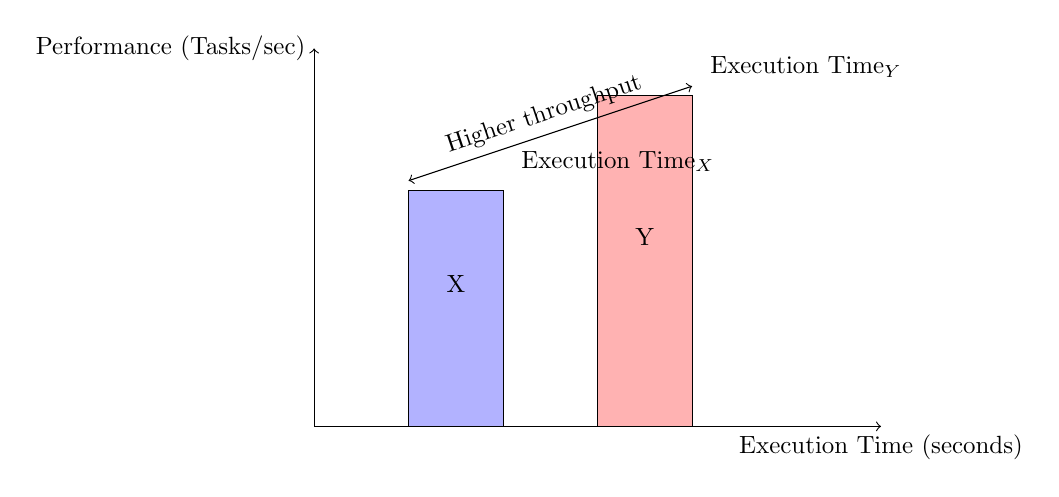
\begin{tikzpicture}[scale=1.2, every node/.style={scale=0.9}]
		% Draw the axes
		\draw[->] (0,0) -- (6,0) node[anchor=north] {Execution Time (seconds)};
		\draw[->] (0,0) -- (0,4) node[anchor=east] {Performance (Tasks/sec)};
		
		% Draw bars for X and Y
		\draw[fill=blue!30] (1,0) rectangle (2,2.5) node[midway, anchor=south, yshift=0.1cm] {X};
		\draw[fill=red!30] (3,0) rectangle (4,3.5) node[midway, anchor=south, yshift=0.1cm] {Y};
		
		% Annotations
		\draw[<->] (1,2.6) -- (4,3.6) node[midway, above, sloped] {Higher throughput};
		\node[anchor=south west] at (2.1, 2.6) {Execution Time$_X$};
		\node[anchor=south west] at (4.1, 3.6) {Execution Time$_Y$};
		
		% Dashed lines for reference
		\draw[dashed] (1,2.5) -- (2,2.5);
		\draw[dashed] (3,3.5) -- (4,3.5);
	\end{tikzpicture}
\end{center}

In this example:
\begin{itemize}
	\item System X has a shorter execution time, indicating higher performance for a given task.
	\item System Y has a longer execution time, leading to lower performance compared to X.
\end{itemize}

\newpage

